\documentclass[10pt]{beamer}

\AtBeginSection[]{
  \begin{frame}
  \vfill
  \centering
  \begin{beamercolorbox}[sep=8pt,center,shadow=true,rounded=true]{title}
    \usebeamerfont{title}\insertsectionhead\par%
  \end{beamercolorbox}
  \vfill
  \end{frame}
}


\usepackage{algorithm,algorithmic}
%\usepackage[noend]{algpseudocode}
%\usepackage{algpseudocode}
\usepackage{tikz}
\usetikzlibrary{bayesnet}
\usetikzlibrary{arrows}
\usepackage{color}
\usepackage{graphicx}
\usepackage{caption}
\usepackage{subcaption}
\usepackage{listings}
\usepackage{bibentry}
\usepackage{natbib}


\title{Latent Dirichlet Allocation}
\author{Jakub Glinka}
\date{March, 2018}
\begin{document}

% -------------------------------------------------->

\begin{frame}
\titlepage
\end{frame}

% -------------------------------------------------->

\section{Model definition}

% -------------------------------------------------->

\begin{frame}
\frametitle{Model definition}

\begin{itemize}
 \item $\theta_{d=1,...,M} \sim \mathrm{Dir}_K(\alpha)$
 \item $\beta_{k=1,...,K} \sim \mathrm{Dir}_V(\eta)$
 \item $z_{d=1,...,M,i=1,...,N_d} \sim \mathrm{Multinomial}_{ \ K}(\theta_d)$
 \item $w_{d=1,...,M,i=1,...,N_d} \sim \mathrm{Multinomial}_{ \ V}(\beta_{z_{di}})$
\end{itemize}

where

\begin{itemize}
 \item $\eta$ is the parameter of the Dirichlet prior on the per-topic word distribution (known and symetric)
 \item $\alpha$ is the parameter of the Dirichlet prior on the per-document topic distributions (known and symetric)
 \item $\theta_d$ is the topic distribution for document d
 \item $\beta_k$ is the word distribution for topic k
 \item $z_{di}$ is the topic for the i-th word in document d
 \item $w_{di}$ is a specific word from d-th document belonging to $V$
\end{itemize}

\end{frame}

% -------------------------------------------------->

\begin{frame}
\frametitle{Model in plate notation}

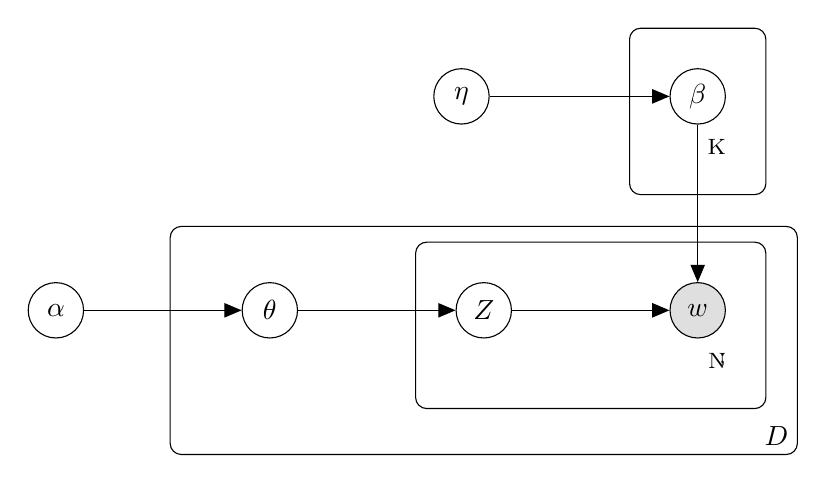
\begin{tikzpicture}

    %nodes
    \node[obs] (w) {$w$};
    \node[latent, above=of w, xshift=-3cm, yshift=1cm] (eta) {$\eta$};
    \node[latent, above=of w, yshift=1cm] (beta) {$\beta$};
    \node[latent, left=of w, xshift=-1cm] (Z) {$Z$};
    \node[latent, left=of Z, xshift=-1cm] (theta) {$\theta$};
    \node[latent, left=of theta, xshift=-1cm] (alpha) {$\alpha$};
    \node [below=of w, xshift=1cm] {$D$};
    
    % edges
    \edge {eta} {beta}  
    \edge {beta} {w}
    \edge {alpha} {theta}  
    \edge {theta} {Z}  
    \edge {Z} {w}  
    
    % plate
    \plate [inner sep=0.5cm, xshift=.0cm, yshift=0.0cm] {plate1} {(beta)} {K}; %
    \plate [inner sep=0.9cm, xshift=.0cm, yshift=-0.2cm] {plate2} {(theta)(Z)(w)}; %
    \plate [inner sep=0.5cm, xshift=.0cm, yshift=0.0cm] {plate3} {(Z)(w)} {N}; %
    
\end{tikzpicture}

\end{frame}


% -------------------------------------------------->

\begin{frame}
\frametitle{Model likelihood}

$$ \log p(z, \theta, \beta, w| \alpha, \eta) = \log p(w|z, \beta) p(z|\theta) p(\theta | \alpha) p(\beta | \eta) = $$
$$ = \log \left( \prod_{k=1}^K p(\beta_k|\eta) \times \prod_{d=1}^D p(\theta_d|\alpha) \times \prod_{d=1}^{D} \prod_{i=1}^{N_d} p(w_{di}|\beta_{z_{di}}) p(z_{di}|\theta_d) \right) = $$
$$ =  \sum_{k=1}^K \log p(\beta_k|\eta) +  \sum_{d=1}^D \log p(\theta_d|\alpha) + \sum_{d=1}^{D} \sum_{i=1}^{N_d} \log p(w_{di}|\beta_{z_{di}}) p(z_{di}|\theta_d) = $$
$$ =  \sum_{k=1}^K \log p(\beta_k|\eta) +  \sum_{d=1}^D \left( \log p(\theta_d|\alpha) + \sum_{i=1}^{N_d} \log p(w_{di}|\beta_{z_{di}}) p(z_{di}|\theta_d) \right) = $$
$$ =  \sum_{d=1}^D \left( \log p(\theta_d|\alpha) + \sum_{i=1}^{N_d} \log \left( p(w_{di}|\beta_{z_{di}}) p(z_{di}|\theta_d) \right) + \frac{1}{D} \sum_{k=1}^K \log p(\beta_k|\eta) \right) $$

\end{frame}

% -------------------------------------------------->

\begin{frame}
\frametitle{Classicial Bayesian Inference}

$$ p(\theta| x) \propto p(x, \theta) = p(x|\theta) p(\theta)$$

\end{frame}

% -------------------------------------------------->

\section{Variational Bayes Inference}

% -------------------------------------------------->


% -------------------------------------------------->

\begin{frame}
\frametitle{Evidence Lower Bound (ELBO)}

$$ \mathcal{L}(x, \phi) := \mathbb{E}_{q}\left[\log p(x, \theta) \right] - \mathbb{E}_{q}\left[\log q(\theta| \phi) \right] $$ \


where $q(\theta|\phi)$ is a parametric approximation of true posterior \footnote{https://en.wikipedia.org/wiki/Variational\_Bayesian\_methods}.

\ \ \
\ \ 

General recipe:

\begin{itemize}
    \item define flexible (and reasonable) family of posterior distributions
    \item derive analytical form of $\mathcal{L}(x, \phi)$
    \item group independent parameters
    \item find coordinate ascent updates 
\end{itemize}



\end{frame}

% -------------------------------------------------->

\begin{frame}
\frametitle{LDA ELBO}

From the definition of the \textbf{E}vidence \textbf{L}ower \textbf{B}ound:

$$ \mathcal{L}(w, \phi, \gamma, \lambda) := \mathbb{E}_{z, \theta, \beta}\left[\log p(w, z, \theta, \beta| \alpha, \eta) \right] - \mathbb{E}_{z, \theta, \beta}\left[\log q(z, \theta, \beta) \right]$$

with posterior of the form

$$q(z, \beta, \theta) = \prod_d \prod_i q(z_{di}) \times \prod_d q(\theta_d) \times \prod_k q(\beta_k)$$

where \footnote{i.e. full factorial design.}

\begin{itemize}
    \item $q(z_{di}) = p(z_{di}|\phi) = \mathrm{Multinomial}_{ \ K}(\phi_{dw_{di}}) $
    \item $q(\theta_d) = p(\theta_d|\gamma) = \mathrm{Dir}_{K}(\gamma_{d}) $
    \item $q(\beta_k) = p(\beta_k|\lambda) = \mathrm{Dir}_{V}(\lambda_{k}) $  
\end{itemize}

\end{frame}

% -------------------------------------------------->

\begin{frame}

\begin{center}
    20 painfull hours later...*
\end{center}



\end{frame}

% -------------------------------------------------->

\begin{frame}
\frametitle{ELBO coordiate ascent algorithm}

\begin{algorithm}[H]
\begin{algorithmic}[1]

\WHILE{improvement $ \mathcal{L}(w, \phi, \gamma, \lambda) > \epsilon$ }
    \WHILE{change $ \gamma > \epsilon $}
        \STATE \emph{E-Step}:
        \FOR{$d \in 1,...,D$}
            \STATE $\phi_{dvk} \propto \exp \left\{ \mathbb{E}_{\beta} \left[ \log \beta_{k v} \right] + \mathbb{E}_{\theta} \left[ \log \theta_{d k} \right] \right\}$
            \STATE $\gamma_{dk} = \alpha_k  + \sum_{v=1}^V n_{dv} \phi_{dvk}$
        \ENDFOR 
        
    \ENDWHILE
    \STATE \emph{M-Step}:
    \STATE $\lambda_{kv} = \eta_v + \sum_{d=1}^D n_{dv}\phi_{dvk}$
\ENDWHILE

\end{algorithmic}
\caption{coordinate ascent VB algorithm for LDA}
\label{alg:seq}
\end{algorithm}

\end{frame}


\section{Implementation}

% -------------------------------------------------->

\begin{frame}

\begin{center}
    Jupyter notebook
\end{center}

\end{frame}

% -------------------------------------------------->


\begin{frame}
\frametitle{References}
\footnotesize{
\begin{thebibliography}{99} % Beamer does not support BibTeX so references must be nserted manually as below
\bibitem[Hoffman, 2010]{p1} Andrew Ng et al. (2003)
\newblock Latent Dirichlet Allocation
\newblock \emph{Journal of Machine Learning Research} 3 (2003) 993-1022

\bibitem[Ng, 2003]{p1} Matthew Hoffman (2010)
\newblock Online Learning for Latent Dirichlet Allocation
\newblock \emph{Advances in Neural Information Processing Systems 23} 


\end{thebibliography}
}
\end{frame}

\end{document}
